%*******************************************************
% Capitulo cuatro
%*******************************************************

\chapter{Propuesta metodológica de producción}

El siguiente capítulo describe las dos categorías más fuertes en metodologías de desarrollo de software y realiza un análisis de las caracteristicas que afectan la decisión de escoger una u otra. Al final se plantean alternativas de selección a la metodología y se discute su escenario de aplicación.

\section{Potenciales metodologías de construcción de software}

Se realizará la construcción de una pieza software para el caso de estudio descrito en el capítulo \ref{Caso_de_estudio}. Este caso de estudio tiene las siguientes restricciones en su proceso de producción:

\begin{itemize}
  \item
\end{itemize}

Toma de decisiones acerca de la producción

Alcance tiempo costo en esta intervención artísticas

Alcance tiempo costo en el caso de estudio

\subsection{Metodologías duras}

Antes de la aparición de las metodologías ágiles dominaban las metodologías que tenían las siguientes características,

\begin{itemize}
  \item Orientación al control del riesgo por iteraciones
  \item Centradas en el diseño
  \item xx
\end{itemize}

La metodología usada en el

Caracteristicas vs creación artística

\subsection{Metodologías ágiles}

Caracteristicas vs creación artística

\section{Selección de la metodología}

Se describe cual adaptación se realiza.










\begin{figure}[h]\label{togafarchimate}
\centering
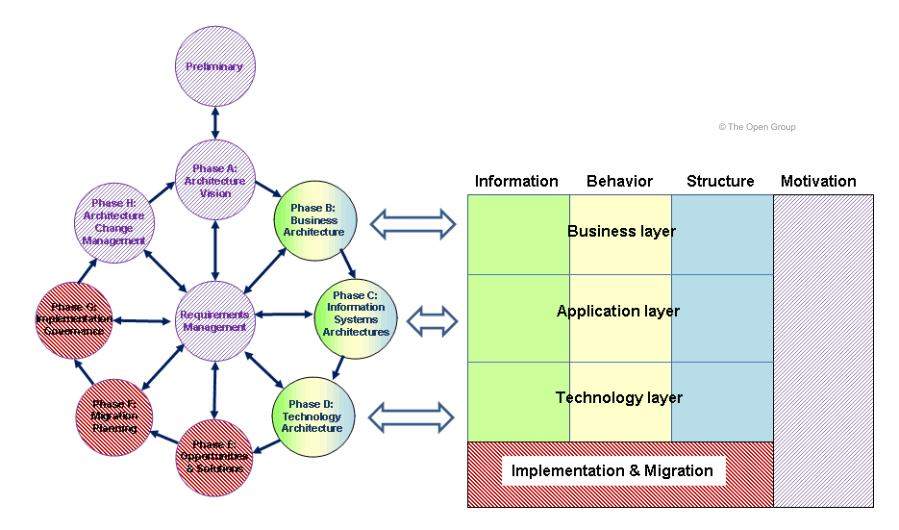
\includegraphics[scale=0.8]{togafarchimate}
\caption{Correspondencia entre Archimate y TOGAF.}
\end{figure}
